\documentclass{article}

\usepackage[portuguese]{babel}

\usepackage[letterpaper,top=2cm,bottom=2cm,left=3cm,right=3cm,marginparwidth=1.75cm]{geometry}
\usepackage[portuguese]{babel}
\usepackage[letterpaper,top=2cm,bottom=2cm,left=3cm,right=3cm,marginparwidth=1.75cm]{geometry}
\usepackage{amsmath}
\usepackage{graphicx}
\usepackage{titling}
\usepackage[colorlinks=true, allcolors=blue]{hyperref}
\usepackage{hyphenat}
\usepackage[utf8]{inputenc}
\usepackage[T1]{fontenc}
\usepackage[official]{eurosym}
\usepackage{fourier}
\usepackage{tikz}
\usepackage[colorlinks=true, allcolors=blue]{hyperref}
\usetikzlibrary{arrows,%
                shapes,positioning}
\renewcommand\maketitlehooka{\null\mbox{}\vfill}
\renewcommand\maketitlehookd{\vfill\null}

\usepackage{listings}
\usepackage{xcolor}
\usepackage{multicol}

\definecolor{codegreen}{rgb}{0,0.6,0}
\definecolor{codegray}{rgb}{0.5,0.5,0.5}
\definecolor{codepurple}{rgb}{0.58,0,0.82}
\definecolor{backcolour}{rgb}{0.97,0.97,0.97}

\usepackage[colorlinks=true, allcolors=blue]{hyperref}
\usetikzlibrary{arrows,%
                shapes,positioning}
\renewcommand\maketitlehooka{\null\mbox{}\vfill}
\renewcommand\maketitlehookd{\vfill\null}


\lstdefinestyle{mystyle}{
    backgroundcolor=\color{backcolour},   
    commentstyle=\color{codegreen},
    keywordstyle=\color{blue},
    numberstyle=\tiny\color{codegray},
    stringstyle=\color{orange},
    basicstyle=\ttfamily\footnotesize,
    breakatwhitespace=false,         
    breaklines=true,                 
    captionpos=b,                    
    keepspaces=true,                
    showspaces=false,                
    showstringspaces=false,
    showtabs=false,                  
    tabsize=2
}

\lstset{style=mystyle}

\begin{document}

\begin{titlepage}
    \begin{center}
    
        \begin{center}
            
\includegraphics[scale=4]{Images/logo-ipp.png}
        \end{center}
    
        \vspace*{6cm}
        
        \LARGE   
        \textbf{Trabalho Prático de Processamento Estruturado de Informação}
            
        \vspace{0.5cm}
        
        Licenciatura em Segurança Informática em Redes de Computadores
        
        \vspace{0.5cm}
        
        \large  
        Janeiro de 2022\\
        
        \vspace{0.5cm} 
        
        \large
        Docentes: \\
        Prof. Bruno Oliveira \\
        Prof. Mariana Carvalho\\
        \vfill
        \vspace{0.8cm}
            
        \large
        Grupo 24     \\
        Gonçalo Pedro Gil, 8200335\\
        Luís Miguel Pires Da Costa, 8200737\\
    \end{center}
\end{titlepage}

\newpage
\section{Índice}

\begin{itemize}
    \item Introdução
        \subitem Contextualização \hspace*{\fill} 2
        \subitem Objetivos do trabalho \hspace*{\fill} 2
        \subitem Breve descrição do trabalho \hspace*{\fill} 2
    \item XML Schema
        \subitem Propriedades   \hspace*{\fill} 3
            \subsubitem Elementos desenvolvidos   \hspace*{\fill} 3
            \subsubitem Atributos   \hspace*{\fill} 4
            \subsubitem Restrições   \hspace*{\fill} 4
            \subsubitem Namespaces   \hspace*{\fill} 4
    \item REST API \hspace*{\fill} 5
    \item XML to JSON \hspace*{\fill} 5
        \subitem Postman   \hspace*{\fill} 6
        \subitem Script em Python   \hspace*{\fill} 6
    \item Consultas MongoDB \hspace*{\fill} 7  
    \item Análise crítica \hspace*{\fill} 8
    \item Conclusão \hspace*{\fill} 9
    \item Bibliografia\hspace*{\fill} 9
\end{itemize} 

\newpage
\section{Introdução}
\subsection{Contextualização}
\hspace{0.5cm}O presente trabalho foi realizado para a disciplina de Processamento Estruturado de Informação na licenciatura de Segurança Informática em Redes e Computadores. \par

\subsection{Objetivos do trabalho}
\hspace{0.5cm}A fim de estudar a criação de vocabulários em XML, o uso de REST API, manipulação de ficheiros JSON e a manipulação de dados em Mongo foi proposto ao grupo a criação de uma API que permitisse o agendamento de visitas e, por fim, a criação de gráficos com as informações recebidas. \par

\subsection{Breve descrição do trabalho}
\hspace{0.5cm}O grupo organizou o trabalho em duas etapas.\par
Numa primeira instância, realizaram-se todos os vocabulários necessários para satisfazer os objetivos do trabalho, de forma a ser possível fazer a validação dos dados antes de serem adicionados na base de dados, e foi efetuada a REST API. \par
Numa segunda etapa, criou-se um script que faz a passagem de documentos XML para documentos JSON e, com esses documentos, foram executadas as querys necessárias para processar toda a informação recebida (algumas foram representadas em forma de gráficos usando o Atlas).  \par

\newpage
\section{XML Schema}
\subsection{Propriedades}
\hspace{0.5cm} Para a concretização do presente projeto, foi indispensável a criação de um XML Schema que cumprisse com os requisitos e objetivos do trabalho, permitindo receber os valores necessários e executar a validação dos mesmos. \par
Este documento é constituído por elementos e os seus atributos, namespaces e restrições. Nos próximos tópicos vão ser descritos e exemplificados todos estes fatores importantes na realização do XML Schema. 

\subsubsection{Elementos  desenvolvidos}
\begin{itemize}
    \item visits: Este trata-se do elemento "root" do documento XML que é constituído por um conjunto de famílias ("family"). De forma a limitar o número existente das mesmas na base de dados, desenvolveu-se um tipo para as "visits" denominado  "VisitsType" (este está explicado em detalhe no tópico "3.1.4 Namespaces" ).
    \item family: Tem como objetivo guardar todas as informações relativas à família e à respetiva reserva, e está restrito a um máximo de sete elementos, devido à impossibilidade de receber famílias com mais de sete elementos. 
    
     \begin{itemize}
         \item number\_members: Representa o número de elementos na família. Criou-se um tipo ("numberType") para ser executável a restrição dos valores inseridos, impossibilitando um input superior a sete,  pelas mesmas razões mencionadas na alínea acima.
         
\begin{lstlisting}[language=XML, caption=numberType]
<xs:simpleType name="numberType">
        <xs:restriction base="xs:integer">
            <xs:pattern value="[1-7]"/>
        </xs:restriction>
    </xs:simpleType>
\end{lstlisting}

         \item member: Tal como o nome indica, caracteriza cada membro da família. Também está  limitado a um máximo de sete ocurrências. Foi criado o "membersType" para este elemento (este está explicado em detalhe no tópico "3.1.4 Namespaces").  
              \subitem nome: Nome do elemento da família
              \subitem data\_nascimento: Data de nascimento do elemento da família, esta é do tipo "date" para possibilitar a validação dos dados introduzidos.
          \item pais: país da família
          \item cidade: cidade da família 
          \item dias\_preferencia: representa os dias em que a família tem disponibilidade para fazer a visita, este está restrito a um máximo de cinco datas a partir de um tipo "preferencesType". 
              \subitem day: dia de preferência, foi criado um tipo ("dayType") de forma a restringir a data ao intervalo de 15-08-2021 a 25-12-2021.

\begin{lstlisting}[language=XML, caption=preferencesType e dayType]
<xs:complexType name="preferencesType">
    <xs:sequence maxOccurs="5">
        <xs:element name="day" type="dayType"/>
    </xs:sequence>
</xs:complexType>

<xs:simpleType name="dayType">
    <xs:restriction base="xs:date">
        <xs:minInclusive value="2021-08-15"></xs:minInclusive> 
        <xs:maxInclusive value="2021-12-25"></xs:maxInclusive> 
    </xs:restriction>
</xs:simpleType>
\end{lstlisting}
     \end{itemize}
\end{itemize}

\subsubsection{Atributos}
\hspace{0.5cm} A fim de ser possível identificar cada família de uma forma única, desenvolveu-se o atributo "ID" (id="5931b18f-9900-4b6d-a7c1-ae3187a8b50c"). Adicionalmente, de forma a ser possível verificar se a visita se encontra apagada ou não, criou-se o atributo "status", que tem como valor default "active"  e, quando apagado, é alterado para "canceled". \par

\begin{lstlisting}[language=XML, caption=Atributos]
    <xs:attribute name="id" type="xs:ID" use="required" />
    <xs:attribute name="status" type="xs:string" default="active" />
\end{lstlisting}


\subsubsection{Restrições}
\hspace{0.5cm} Com o objetivo de validar a informação inserida foram criadas as seguintes restrições:
\begin{itemize}
    \item "preferencesType": restringe a um máximo de cinco datas inseridas
\begin{lstlisting}[language=XML, caption=Restrição preferencesType]
    <xs:complexType name="preferencesType">
        <xs:sequence maxOccurs="5">
            <xs:element name="day" type="dayType"/>
        </xs:sequence>
    </xs:complexType>
\end{lstlisting}

    \item "dayType": limita a data inserida ao intervado de 2021-08-15 a 2021-12-25
\begin{lstlisting}[language=XML, caption=Restrição dayType]
    <xs:simpleType name="dayType">
        <xs:restriction base="xs:date">
            <xs:minInclusive value="2021-08-15"></xs:minInclusive> 
            <xs:maxInclusive value="2021-12-25"></xs:maxInclusive> 
        </xs:restriction>
    </xs:simpleType>
\end{lstlisting}

    \item "numberType": limita o número inserido ao intervalo de 1 a 7
\begin{lstlisting}[language=XML, caption=Restrição numberType]
    <xs:simpleType name="numberType">
        <xs:restriction base="xs:integer"> 
            <xs:pattern value="[1-7]"/>
        </xs:restriction>
    </xs:simpleType>
\end{lstlisting}
\end{itemize}




\subsubsection{Namespaces}
\hspace{0.5cm} Os namespaces são um conjunto de nomes únicos. Um mecanismo pelo qual o elemento e o nome dos atributos podem ser atribuídos a um grupo, sendo identificados pela URI. Assim, para o presente projeto foram criados os seguintes URI:

\begin{itemize}
    \item http://www.oficina.paiNatal.pt/Visits: namespace referente ao xsd schema das "visits"
\begin{lstlisting}[language=XML, caption=XMLSchema Visits]
<xs:schema xmlns:xs="http://www.w3.org/2001/XMLSchema"
           xmlns="http://www.oficina.paiNatal.pt/Visits"
           targetNamespace="http://www.oficina.paiNatal.pt/Visits"
           xmlns:xf="http://www.oficina.paiNatal.pt/Family"
           elementFormDefault="qualified">

        <xs:import schemaLocation="Family.xsd" namespace="http://www.oficina.paiNatal.pt/Family"/>

        <xs:element name="visits">
            <xs:complexType>
                <xs:sequence maxOccurs="5000">
                    <xs:element name="family" type="xf:familyType"/>
                </xs:sequence>
            </xs:complexType>
        </xs:element>

</xs:schema>
\end{lstlisting}
    
    \item http://www.oficina.paiNatal.pt/Family: namespace referente ao xsd schema da "Family"
\begin{lstlisting}[language=XML, caption=XMLSchema Family]
<xs:schema xmlns:xs="http://www.w3.org/2001/XMLSchema" 
        xmlns="http://www.oficina.paiNatal.pt/Family" 
        targetNamespace="http://www.oficina.paiNatal.pt/Family" 
        xmlns:xm="http://www.oficina.paiNatal.pt/Members" 
        elementFormDefault="qualified">

    <xs:import schemaLocation="Members.xsd" namespace="http://www.oficina.paiNatal.pt/Members" />
(...)
</xs:schema>
\end{lstlisting}
    
    \item http://www.oficina.paiNatal.pt/Members: namespace referente ao xsd schema dos "Members"
\begin{lstlisting}[language=XML, caption=XMLSchema Members]
<xs:schema xmlns:xs="http://www.w3.org/2001/XMLSchema"
    xmlns="http://www.oficina.paiNatal.pt/Members"
    targetNamespace="http://www.oficina.paiNatal.pt/Members"
    elementFormDefault="qualified">
    
    <xs:complexType name="memberType">
        <xs:sequence>
            <xs:element name="nome" type="xs:string"/>
            <xs:element name="data_nascimento" type="xs:date"/>
        </xs:sequence>
    </xs:complexType>

</xs:schema>
\end{lstlisting}
\end{itemize}

\section{REST API}
Tal como já anteriormente referido, constatou-se a necessidade de programar uma REST API com as seguintes capacidades: \par
\begin{itemize} 
    \item Visualizar todas as visitas: retorna todas as visitas, já agendadas, presentes na base de dados ("/getvisits");
    \item Visualizar visita em específico: recebe como parâmetro o ID da visita em questão e retorna a informação em XML da mesma ("/getvisit");
    \item Adicionar visitas: recebe um agendamento e valida os dados do mesmo, caso tudo seja válido, atribui-lhe um UID e o status de "active" ("/addvisit");
    \item Cancelar visitas: recebe o ID da visita a cancelar e altera o atributo "status" para "canceled". O grupo optou por esta abordagem para que se  possibilitasse um tratamento dos dados mais rápido e menos custoso para o sistema que o está a processar ("/delvisit").
\end{itemize}

\section{XML para JSON}
\hspace{0.5cm} De forma a poder fazer a integração dos dados na plataforma Atlas, foi necessário fazer a passagem dos dados de XML para JSON. Para tal, foram programadas duas pipelines distintas para satisfazer o mesmo fim, uma primeira bastante semelhante ao que fora lecionado em aula (alínea 5.1) e uma outra usando programação em Python (alínea 5.2).
\subsection{Postman}

\hspace{0.5cm} A partir do diagrama abaixo podemos entender como se comporta a pipeline e todos os processos envolvidos na mesma.
\begin{center}
    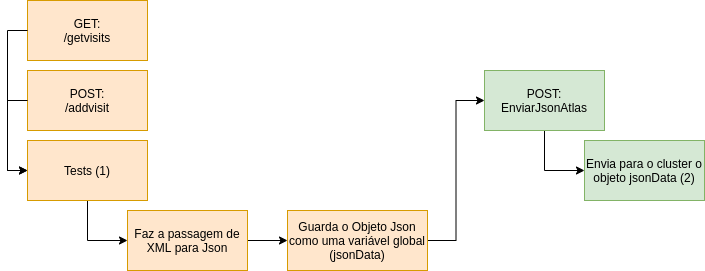
\includegraphics[scale=0.57]{Images/XMLtoJsonDiagram.drawio.png}
\end{center}

\begin{itemize}
    \item 1. Neste primeiro passo utilizou-se a funcionalidade "Tests" do Postman. Esta possibilitou ao grupo programar em JavaScript um pequeno script que passasse a resposta dos pedidos para JSON e, de seguida, guardar esse objeto JSON numa variável global do Postman.
    \item 2. A partir da API do Atlas foi programado um POST que recebe um Objeto JSON e envia-o para o cluster do grupo.
\end{itemize}

\subsection{Script em Python}
\hspace{0.5cm} A pipeline programada em python pode ser facilmente interpretada com o seguinte diagrama:

\begin{center}
    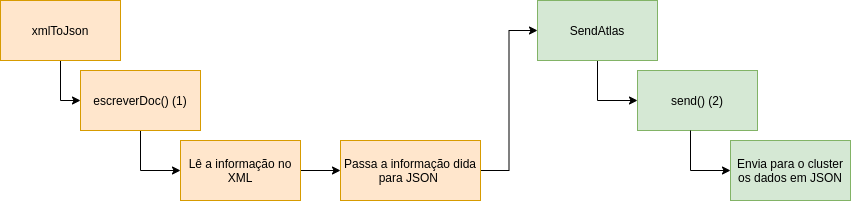
\includegraphics[scale=0.515]{Images/pipelinePython.png}
\end{center}

\hspace{0.5cm}Explicação das tarefas realizadas pela pipeline:
\begin{itemize}
    \item 1. Função responsável pela passagem de XML para JSON, recebendo um documento XML e o diretório de destino para guardar o ficheiro em JSON.
    \item 2. Recebe o diretório do ficheiro JSON anteriormente mencionado e usa a API do Atlas para enviar a informação para o Cluster criado pelo grupo. 
\end{itemize}

\begin{lstlisting}[language=XML, caption=Output]
$ ./xmlToJson.py --help
+ Instruções + 
| xmlToJson_v2.py 'docPath' 'savePath' 
|
| docPath : diretorio do documento xml 
| savePath: diretorio do documento json (valor por defeito ./data.json) 
$ ./xmlToJson.py Visits.xml doc.json
| XML --> JSON         
| Ficheirio guardado com sucesso em: ../JSON/teste.json
{"insertedIds":["61e83017430d032e9090f488","61e83017430d032e9090f489"]}
| JSON --> Atlas         
| Ficheirio enviado com sucesso para: Cluster0 
\end{lstlisting}

\section{Consultas MongoDB}

\begin{itemize}
    \item Apresentar o número total de agendamentos até ao momento
\begin{lstlisting}[language=XML, caption=]
$ db.visits.find().count()
\end{lstlisting}
    \item Apresentar o total de famílias por dia
\begin{lstlisting}[language=XML, caption=]
$ db.visits.aggregate([{"$match":{"f:dias_preferencia.f:day":"2021-12-24"}},{"$count":"2021-12-24"}]).pretty() 
\end{lstlisting}
    \item Apresentar o total de pessoas por dia
\begin{lstlisting}[language=XML, caption=]
$ db.visits.aggregate([{"$match":{"f:dias_preferencia.f:day":"2021-09-02"}},{ "$group":{"_id":"$f:dias_preferencia.f:day", "total_pessoas":{"$sum":{$toInt: "$f:number_members"}}}}])
\end{lstlisting}
    \item A percentagem de ocupação por dia
\begin{lstlisting}[language=XML, caption=]
$ db.visits.aggregate([{"$match":{"f:dias_preferencia.f:day":"2021-12-24"}},{ "$group":{"_id":"$f:dias_preferencia.f:day", "total_pessoas":{"$sum":{$toInt: "$f:number_members"}}}},{"$project":{"_id":0,"total_pessoas": 1, "percentagem_ocup":{$divide:[{ $multiply: [ "$total_pessoas", 100]},50]}}}])
\end{lstlisting}
    \item O número de cancelamentos por dia
\begin{lstlisting}[language=XML, caption=]
$ db.visits.aggregate([{"$match":{"@status":"cancel","f:dias_preferencia.f:day":"2021-12-24"}},{"$count":"cancelados"}])
\end{lstlisting}
    \item Por cidade e por país, apresentar o número de agendamentos
\begin{lstlisting}[language=XML, caption=]
$ db.visits.aggregate([{"$match":{"f:pais":"Portugal","f:cidade":"Lisboa"}},{"$count":"family"}]).pretty()
\end{lstlisting}
\end{itemize}

\newpage
\section{Análise crítica}

\hspace{0.5cm} Para o presente trabalho começou-se por desenvolver todos os meios de validação dos dados/ficheiros XML. Para isso, foram desenvolvidos XML schemas com a função de validar e restringir os dados inseridos pelos utilizadores. Adicionalmente, foram, também, usados namespaces de forma a ser possível deter vários ficheiros, cada um com validações de dados diferentes, tendo assim um código mais organizado e de possível reutilização. Desta forma, conseguimos obedecer a todos os requisitos do projeto referentes a todas as restrições dos dados, como por exemplo, o número máximo de elementos na família (7) e o número máximo de marcações possíveis (5000). \par
De seguida, começou-se a programar uma REST API que possibilitasse a procura, cancelamento e agendamento de visitas. Este passo foi de complexa execução devido a dois fatores predominantes, a falta de documentação do BaseX e de conhecimentos por parte dos elementos do grupo. Contudo, o grupo foi capaz de aprender e adquirir os conhecimentos necessários para a programação desta API e de todas as capacidades solicitadas nos objetivos do projeto, de forma autodidata. Adicionalmente, a API também é responsável pela atribuição dos UID de todas as marcações.\par
Uma vez tendo a capacidade de validação dos valores dos clientes (XML Schema) e de criar, remover e visualizar os agendamentos a partir de uma API, já foi possível dar início à segunda fase do projeto. \par
Esta tem como principais objetivos fazer a passagem dos dados em XML para JSON, programar algumas querys em MongoDB que possibilitassem a análise dos dados e, por fim, a partir da plataforma Atlas, fazer a demonstração gráfica dos dados inseridos. \par
Assim, começou-se por criar um script em python que recebesse um ficheiro em XML e efetuasse a passagem desses dados para JSON (gravando os mesmos num documento). De forma a poder aprimorar um pouco os resultados do script teve-se o cuidado de formatar o output, possibilitando assim uma melhor compreensão e apresentação dos resultados. De seguida, é realizado o envio da informação JSON criada para o Cluster do grupo na plataforma Atlas a partir da API da mesma. \par
De forma a usar os conhecimentos adquiridos em aula, foi criada uma segunda pipeline que, mais uma vez, passasse os dados de XML para JSON e enviasse os mesmos para o Atlas. Esta foi feita na sua totalidade no Postman, tendo sido programado em JavaScript um pequeno script que recebe o output de um GET request e passa o mesmo para JSON, guardando este numa variável global ( "jsonData").  Por fim, é realizado um POST ao Cluster do grupo usando a API do Atlas onde são enviadas as informações que foram guardadas na variável.\par
Para terminar, com este documento JSON o grupo pôde começar a criar as querys para a análise dos dados, tal como os gráficos de visualização no Atlas.


\newpage
\section{Conclusão}
\hspace{0.5cm} Este trabalho cumpriu com todos os objetivos iniciais, tanto a nível dos objetivos propostos, como a nível das competências desenvolvidas pela execução dos mesmos. \par
O grupo teve a oportunidade de estudar aprofundadamente um ambiente mais prático da área da programação de sistemas e APIs usando XML, tal como a criação de bases de dados em Mongo usando ficheiros JSON (envolvendo pesquisa, pensamento crítico e formulação).
Podemos certamente afirmar que todo o trabalho e dedicação empregues neste projeto foram altamente enriquecedores em inúmeras áreas, desde o trabalho em equipa, à escrita de um relatório técnico, até ao estudo autónomo por parte dos elementos do grupo. \par
Por fim, é seguro afirmar que acabamos este projeto mais enriquecidos e preparados para o restante percurso académico e mundo profissional. \par

\section{Bibliografia}
\begin{itemize}
    \item https://docs.basex.org/wiki/Main\_Page
    \item https://docs.basex.org/wiki/REST
    \item https://docs.mongodb.com/
    \item Powerpoints da disciplina
\end{itemize}
\end{document}